\documentclass[tikz]{standalone}
\begin{document}

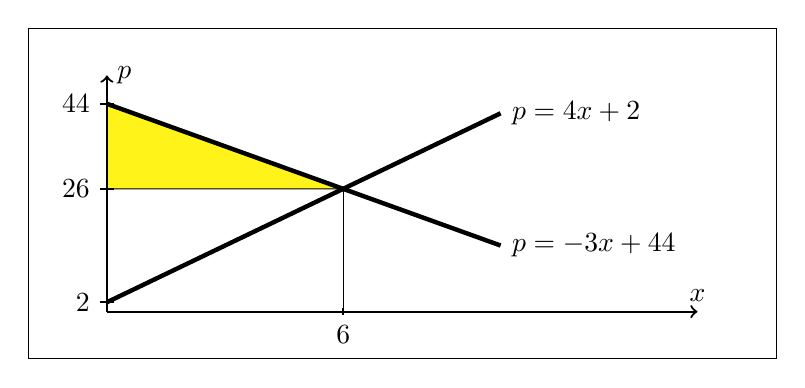
\begin{tikzpicture}[scale=0.5,yscale=0.12]

  \draw[fill=white] (-2,-10) rectangle ++(19,70);

  % shade region
  \draw[fill=yellow!90] plot[smooth, samples=10, domain=0:6] (\x,44 - 3*\x) -| (0,44);
    
  % draw axes 
  \draw[thick,->] (0,0) -- (15,0) node[above] {$x$};
  \draw[thick,->] (0,0) -- (0,50) node[right] {$p$};
    
  % draw curve
  \draw[ultra thick,domain=0:10,samples = 100, smooth,variable=\x,black] plot ({\x},{44 - 3*\x}) node[right] {$p=-3x+44$};
  \draw[ultra thick,domain=0:10,samples = 100, smooth,variable=\x,black] plot ({\x},{2 + 4*\x}) node[right] {$p=4x+2$};

  % tick marks
  \foreach \x in {6} 
    \draw [thick] (\x cm,20pt) -- (\x cm,-20pt) node[below] {\x};
  \foreach \y in {2,26,44} 
    \draw [thick] (5pt,\y cm) -- (-5pt,\y cm) node[left] {\y};

  \draw (6,26) -- (6,0);
  %      \draw (6,26) -- (0,26) node[left] {$\Bar{p}$};
  %      %\draw[<-] (0.4,2) -- (1.5,3) node[right] {Consumer Surplus};
\end{tikzpicture}
\end{document} 
